\section{Results}

In order to test our results, we have built a testing framework. The requirements for this were, that it should allow us to quickly and accurately evaluate changes to the detection algorithms. Manual testing is good, but requires us to manually select a sequence and a frame, which can get tedious very quickly.

To combat this, and also get more consistent results, we have defined an array of representative frames from each sequence. We have carefully selected the frames which we had found to cause most problems for our detection algorithms during manual testing. Therefore our representative sample contains the worst-case frames for each sequence (eye looking different directions, challenging light, or eye position). 

On the other hand, we have selected only 5-8 frames per sequence (56 frames together), so the testing can quickly finish and produce representative results. We have also made sure that all of the frames in question do contain the pupil (i.e no frames with closed eye or where no detection can be made) The testing script also writes all the frames with pupil/iris/glint detections drawn on top into a folder for further (manual) inspection.

Unfortunately we cannot automatically test if a detection is correct, because we have no reference implementation, so the correction still has to be evaluated manually. But what we can detect automatically is the number of detected results (i.e what percentage of images that contained eye have had at least something detected by our implementation). This can at least give us  at least preliminary results, if we assume that most of the detected pupils are correct, we should get a good idea about the results from this alone. Of course this does not mean that we can solely rely on this automatic testing and therefore manual verification still has to be performed.

\begin{table}[h!]
	\center
	\begin{tabular}{ |l|l|l|l| }
		\hline
		Sequence & Frames Evaluated & Pupil Detected & Detected Correctly \\ \hline
		
		eye1.avi 	& 5 	& 5 (100\%)	& 5 (100\%) \\
		eye2.avi 	& 6 	& 6 (100\%)	& 6 (100\%) \\
		eye3.avi 	& 8 	& 8 (100\%)	& 5 (62.5\%) \\
		eye4.avi 	& 8 	& 6 (75\%)	& 6 (75\%) \\
		eye5.avi 	& 6 	& 5 (83.3\%)	& 2 (33.3\%) \\
		eye6.avi 	& 7 	& 7 (100\%)	& 5 (71.43\%) \\
		eye7.avi 	& 8 	& 8 (100\%)	& 8 (100\%) \\
		eye8.avi 	& 8 	& 5 (62.5\%)	& 5 (62.5\%) \\
		
		\hline
		Total 	& 56 & 50 (89.29\%) & 42 (75\%) \\ 
		\hline
	\end{tabular}
	\caption{Semi-Automatic Evaluation of the Detection Algorithm}
	\label{tab:eval}
\end{table}

The Table \ref{tab:eval} shows how many frames were evaluated per sequence, how many of those frames have had something detected by our algorithm (counted automatically during testing) and lastly, how many of the frames have the pupil detected correctly \footnote{By definition of our sample, all frames have the pupil present, so it is an error of the algorithm if it is not detected} (this has been done by manual inspection of all generated frames, i.e pupil detected is right size and corresponds to the actual location of the pupil in the image). 

\begin{figure}[t]
	\centering
	
	\begin{subfigure}[b]{0.5\textwidth}
		\centering
		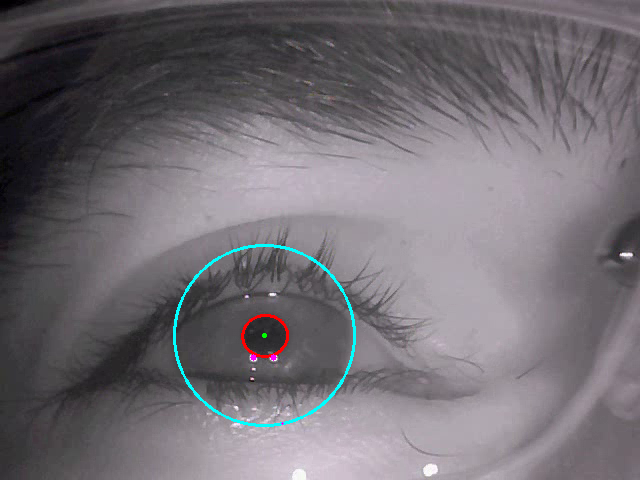
\includegraphics[width=\textwidth]{Handin1/images/good1.png}
		\caption{Eye Squinting}
		\label{subfig:squinting}
	\end{subfigure}%
	~
	\begin{subfigure}[b]{0.5\textwidth}
		\centering
		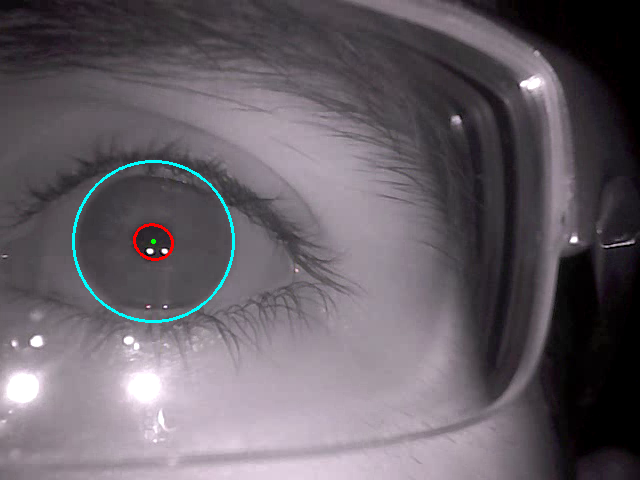
\includegraphics[width=\textwidth]{Handin1/images/good2.png}
		\caption{Challenging Light}
		\label{subfig:challenging_light}
	\end{subfigure}
	
	\begin{subfigure}[b]{0.5\textwidth}
		\centering
		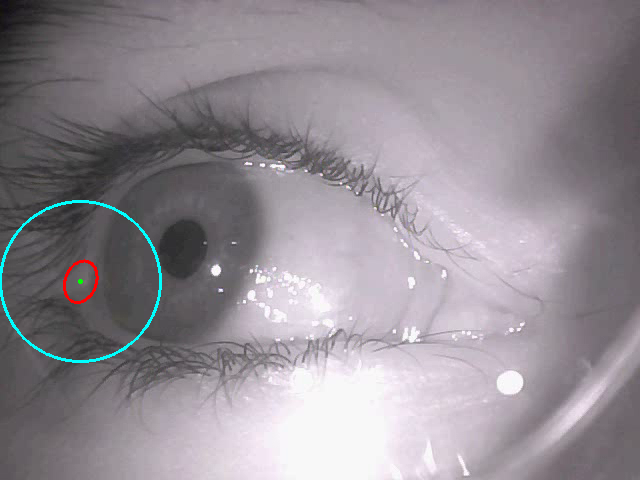
\includegraphics[width=\textwidth]{Handin1/images/wrong1.png}
		\caption{Wrong Detection}
		\label{subfig:wrong1}
	\end{subfigure}%
	~
	\begin{subfigure}[b]{0.5\textwidth}
		\centering
		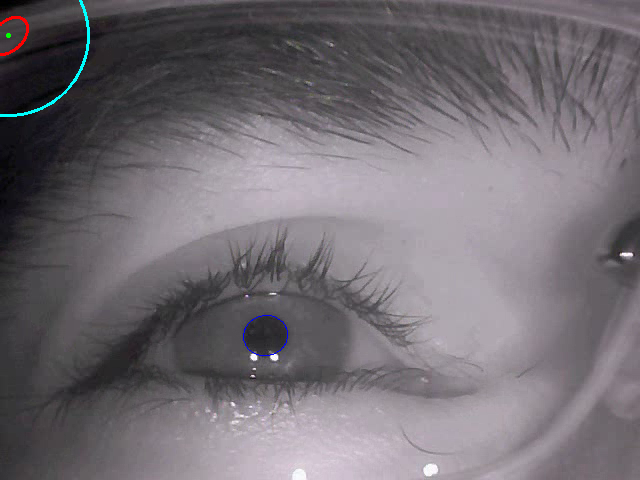
\includegraphics[width=\textwidth]{Handin1/images/wrong2.png}
		\caption{Ordering By Extend}
		\label{subfig:extend}
	\end{subfigure}
	
	\caption{Results}
	\label{fig:results}
\end{figure}

Figure \ref{fig:results} shows good results in the first row (images (a) and (b)) under challenging conditions, as well as wrong results that can occur in row two (images (c) and (d)). In Figure \ref{subfig:extend} you can see a blue circle around the pupil, which is an alternative blob that has been considered by the algorithm, but was most likely rejected because the closing in combination with glints have increased its extend in comparison with the other candidate.

\subsection{Discussion}
In the following text we look at the weaknesses of our algorithm, why it does not work in all frames, and how it could be improved. We look at three interesting points of view from which the work could be improved. First we look at performance, where we evaluate what could be done better to improve performance, second and third we discuss false positives and negatives, which occurred during our testing, what reasons there were for this and how could the algorithm be improved.

\subsubsection{Performance}
Regarding performance, our algorithm is not achieving very good results, primarily because we focused on the detection and code readability, and due to shortage of time we could not work on the speed optimizations as we would have liked. However we can mention some of the sacrifices we have made to improve code readability and ease of handling during testing. 
For example in various parts of the algorithm we use the gray scale image, which we most of the time just calculate again, instead we could either implement some sort of cache or pass the gray scale image around and only generate it once. Similar story is with k-means image. We use the same algorithm in pupil and glint detection, yet these two don’t share the results, which they should.

\subsubsection{False Positives}
False positives are cases where a pupil is detected in a place where it is not actually supposed to be. We have found that this usually occurs when there are very dark areas in the image. This confuses the k-means, producing the darkest region that does not necessarily contain the pupil, at which point the whole algorithm is destined to fail. It will pick a blob that best resembles the pupil out of those available and try to work with that, producing wrong results. 
A solution we have tried to combat this problem is overlaying a transparent-to-white radial gradient from the center of the image to suppress the dark areas around image edges. But what we found was that even though the number of detections in sequences that were most affected by the above described problem went up, the overall results over all of the sequences were worse. So we decided against that improvement. However it still might be warranted to selectively apply it to only some of the sequences, if it can be safely assumed that the pupil stays near the center of the frame and there are dark areas near the edges of the frame.

\subsubsection{False Negatives}
False negatives are produced when a pupil should have been detected, but was not. These cases can be caught by our automated testing, because all of the frames being tested should contain a pupil. This is of course very similar to the previous case with k-means, but we have to manage limiting this problem using the iterative lowering of k-means parameter.
